\chapter{Eksperimen dan Pembangunan Sistem}

\section{Lingkungan Eksperimen dan Pembangunan Sistem}

Eksperimen dilakukan di platform \href{https://www.kaggle.com}{Kaggle} dengan Kernel. Bahasa Pemrograman yang digunakan adalah bahasa Python versi 3.6.6. Pada \textit{fine-tuning} layer terakhir digunakan CPU 1xSingle core hyper threaded Xeon Processors @2.3Ghz, 46MB Cache. Pada \textit{fine-tuning} penuh digunakan TPU v3-8. Eksperimen dikembangkan menggunakan kombinasi pustaka PyTorch \parencite{paszke2017automatic}, TensorFlow \parencite{tensorflow2015}, dan HuggingFace \parencite{HuggingFace}.

Pada eksperimen fine-tuning layer terakhir, pengembangan dilakukan menggunakan pustaka PyTorch. Dikarenakan model belum terdapat di pustaka HuggingFace pada saat pengembangan,ekstraksi fitur dilakukan dengan mengakses fungsi di \textit{repository} resmi XLM Facebook\footnote{\url{https://github.com/facebookresearch/XLM}}. Agar tidak mengulangi pengektraksian fitur pada tiap eksperimen, seluruh fitur diekstrak terlebih dahulu dan disimpan dalam bentuk NumpyArray \parencite{numpy}. Selain itu, untuk memastikan bahwasanya eksperimen \textit{reproducible} dan tidak memiliki faktor acak, semua opsi \textit{seed} baik di System, Python, hingga pustaka Pytorch ditetapkan agar hasil tidak berubah jika eksperimen dijalankan berkali-kali dengan kondisi yang sama. Hasil akhir eksperimen fine-tuning layer terakhir adalah rata-rata dari 6 eksperimen dengan \textit{seed} dari 1-6.

\begin{lstlisting}[language=Python]
def set_seed():
    seed=1
    random.seed(seed)
    torch.manual_seed(seed)
    torch.cuda.manual_seed_all(seed)
    np.random.seed(seed)
    os.environ['PYTHONHASHSEED'] = str(seed)
    torch.backends.cudnn.deterministic = True
\end{lstlisting}

Pada eksperimen fine-tuning penuh, pengembangan dilakukan menggunakan TensorFlow dan HuggingFace. Hal ini dikarenakan pada saat pengembangan, TPU dapat lebih mudah dimanfaatkan dengan pustaka TensorFlow. Dikarenakan sifat dari TPU yang \textit{asynchronous}, menjalankan model berkali-kali akan menghasilkan nilai yang sedikit berbeda. Meski begitu, perbedaan tidak terlalu jauh sehingga kesimpulan tetap dapat diambil.


\section{Eksperimen}
Eksperimen dilakukan dengan 2 model multilingual (XLM-R \& Multilingual BERT). Pada tiap eksperimen dilakukan variasi total data (500/1000/2500/5000/7500/MAX) dan kelipatan bahasa asing (0.25/0.5/0.75/1/1.5/2/3/4/5/6/7/8/9/10) pada skenario \textit{multilingual learning}. Untuk konfigurasi model, digunakan callback berupa EarlyStopping dan ReduceLROnPlateau. Penggunaan callback EarlyStopping digunakan agar model tidak overfit. Sedangkan callback ReduceLROnPlateau digunakan untuk membantu model mencapai performa yang lebih baik. Semua eksperimen dijalankan hingga diberhentikan oleh callback EarlyStopping.

Pada eksperimen fine-tuning layer terakhir, dipilih probabilitas \textit{dropout} 0.2, \textit{learning rate} 1e-3, \textit{patience} callback ReduceLROnPlateau 5, dan \textit{patience} callback EarlyStopping 12. Sedangkan pada eksperimen fine-tuning penuh, dipilih probabilitas \textit{dropout} 0.2, \textit{learning rate} 1e-5, \textit{patience} callback ReduceLROnPlateau 0, dan \textit{patience} callback EarlyStopping 4. Dapat dilihat pemilihan \textit{hyperparamter} yang lebih agresif pada eksperimen fine-tuning layer terakhir. Besar \textit{learning rate} 1e-5 fine-tuning penuh ini berdekatan dengan anjuran besar \textit{learning rate} fine-tuning penuh penelitian \parencite{Devlin_Chang_Lee_Toutanova_2019}. Untuk \textit{learning rate} fine-tuning layer terakhir, hal ini mengikuti \parencite{Peters_Ruder_Smith_2019} yang mendukung penggunaan learning rate lebih besar di layer yang lebih akhir. 

Pada tiap eksperimen, data \textit{train} akan dipisah menjadi data latih dan validasi dengan besar pembagian 9:1. Pada tiap epoch, model dilatih pada bagian data latih dan divalidasi pada bagian data validasi. Tergantung dengan performa dari validasi tadi, model akan menentukan apakah pelatihan akan dilanjutkan, \textit{learning rate} diturunkan, atau pelatihan diberhentikan. Pada akhir pelatihan, model dengan performa pada data validasi terbaik akan digunakan untuk memprediksi data uji.

    \subsection{Hasil fine-tuning layer terakhir model XLM-R}
        Berikut hasil eksperimen \textit{fine-tuning} layer terakhir dengan model XLM-R: 
        \begin{enumerate}
            \item \textbf{Analisis sentimen dengan data dataset A} \\
            Gambar \ref{fig:plot_head_trip_xlmr} adalah rangkuman dari seluruh eksperimen pada fine-tuning layer terakhir dataset ini. Pada sumbu X, terdapat informasi mengenai skenario dari eksperimen. Paling kiri dan ditandai dengan titik warna merah adalah hasil skenario zero-shot. Setelah itu ditandai dengan titik warna hijau adalah skenario monolingual. Seterusnya ke kanan adalah skenario multilingual dengan data bahasa Inggris ditambah. Pada sumbu Y terdapat informasi mengenai performa model. 

            \begin{figure}[ht]
                \centering
                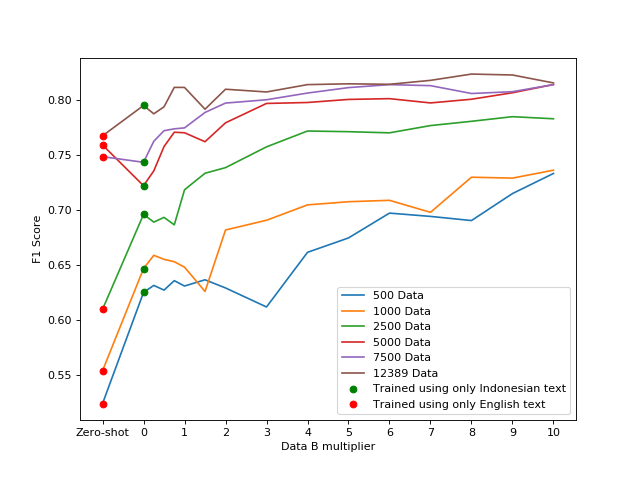
\includegraphics[width=0.9\textwidth]{resources/plot-head-trip-xlmr.png}
                \caption{Plot dataset A dengan model XLM-R}
                \label{fig:plot_head_trip_xlmr}
            \end{figure}

            Dapat dilihat pada Gambar \ref{fig:plot_head_trip_xlmr}, performa analisis sentimen dataset A terbantu dengan penambahan data berbahasa Inggris. Di berbagai total data, penambahan bahasa Inggris menambah rata-rata F1-score sebesar 0.106 dari baseline monolingual. Penambahan performa terbesar juga diobservasi pada eksperimen dengan jumlah data yang sedikit. Performa model pada kasus 500 data meningkat dari baseline monolingual sebesar 0.484 ke 0.682 pada multilingual learning dengan 10x data bahasa Inggris. Performa model tertinggi, F1-score 0.808, datang dari penambahan bahasa Inggris sebanyak 9 kali lipat dari total bahasa Indonesianya.

            \item \textbf{Analisis sentimen dengan dataset B} \\
            Dapat dilihat pada Gambar \ref{fig:plot_head_prosa_xlmr}, performa analisis sentimen dataset B sangat terbantu dengan penambahan data berbahasa Inggris. Di berbagai total data, penambahan bahasa Inggris menambah rata-rata F1-score sebesar 0.179. Penambahan performa terbesar juga diobservasi pada eksperimen dengan jumlah data yang sedikit. Performa model pada kasus 1000 data meningkat dari baseline monolingual sebesar 0.424 ke 0.717 pada multilingual learning dengan 10x data bahasa Inggris. Performa model tertinggi, F1-score 0.795, datang dari penambahan bahasa Inggris sebanyak 9 kali lipat dari total bahasa Indonesianya.

            \begin{figure}[ht]
                \centering
                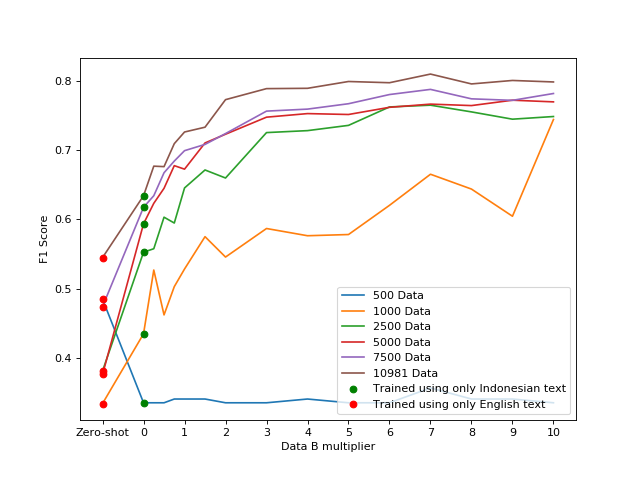
\includegraphics[width=0.9\textwidth]{resources/plot-head-prosa-xlmr.png}
                \caption{Plot dataset B dengan model XLM-R}
                \label{fig:plot_head_prosa_xlmr}
            \end{figure}

         
            \item \textbf{Klasifikasi ujaran kebencian \& kasar} \\
            Dapat dilihat pada Gambar \ref{fig:plot_head_toxic_xlmr}, performa klasifikasi ujaran kebencian tidak terlalu terbantu dengan penambahan data berbahasa Inggris. Performa model sempat terbantu, namun penambahan lebih banyak data bahasa Inggris menurunkan performa model. Meski begitu, pada kasus data yang sedikit (500, 1000, dan 2500 data) \textit{multilingual learning} berhasil meningkatkan performa model. Data dilihat peningkatan terbesar pada data sebanyak 500 di mana performa F1-score baseline monolingual sebesar 0.363 meningkat ke 0.641 di \textit{multilingual learning} dengan besar kelipatan bahasa Inggris 10 kali lipat.

            \begin{figure}[ht]
                \centering
                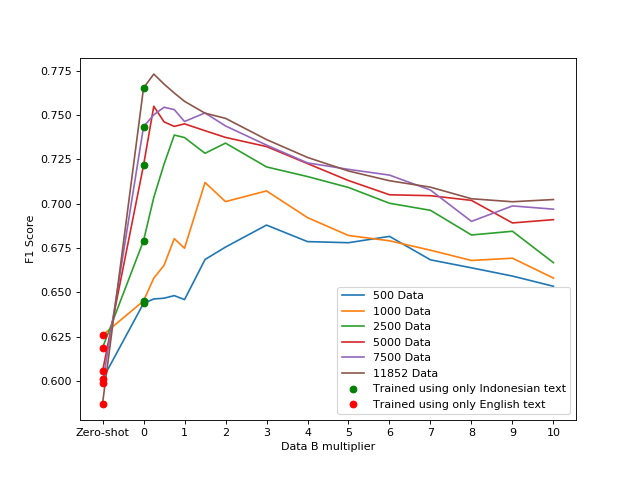
\includegraphics[width=0.9\textwidth]{resources/plot-head-toxic-xlmr.png}
                \caption{Plot klasifikasi ujaran kebencian dengan model XLM-R}
                \label{fig:plot_head_toxic_xlmr}
            \end{figure}

        \end{enumerate}

        Melalui rangkaian eksperimen \textit{fine-tuning} hanya layer terakhir model XLM-R di atas, dapat diobservasi beberapa fenomena. Pertama, penambahan data bahasa Inggris dapat meningkatkan performa dalam klasifikasi teks bahasa Indonesia. Peningkatkan performa juga diobservasi lebih efektif dalam data yang berjumlah lebih sedikit. Namun, ada kasus di mana penambahan data malah menurunkan performa. Analisis lebih dalam diperlukan untuk mengetahui penyebab terjadinya fenomena tersebut.

        \begin{figure}[htb]
            \centering
            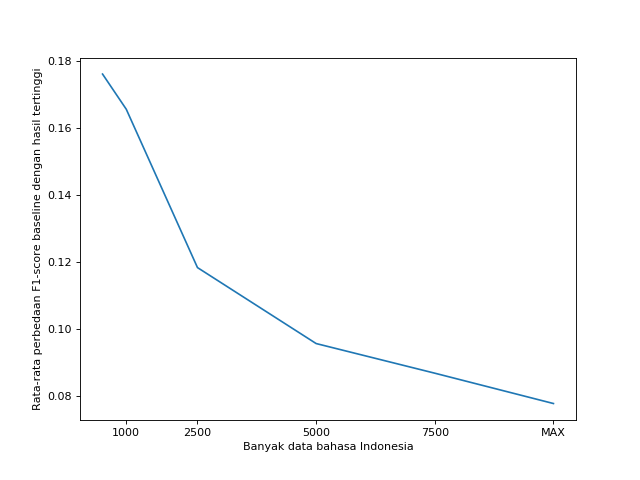
\includegraphics[width=0.9\textwidth]{resources/plot-gain-xlmr.png}
            \caption{Plot rata-rata kenaikkan performa model XLM-R}
            \label{fig:plot_gain}
        \end{figure}

        Dengan merata-ratakan perbedaan antara nilai baseline monolingual dengan hasil tertinggi skenario \textit{multilingual learning}, dapat dilihat dengan jelas efek penambahan data bahasa Inggris lebih tinggi di eksperimen dengan data bahasa Indonesia lebih sedikit. Hal ini menunjukkan bahwasanya teknik ini lebih efektif jika jumlah data sedikit. Plot rata-rata dapat dilihat pada gambar \ref{fig:plot_gain}

    \subsection{Hasil fine-tuning layer terakhir model mBERT}
        Berikut hasil eksperimen \textit{fine-tuning} layer terakhir dengan model mBERT: 
        \begin{figure}[htb]
            \minipage{0.33\paperwidth}
            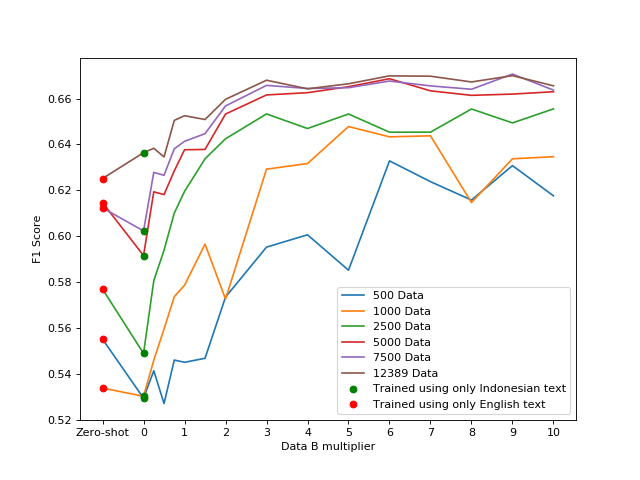
\includegraphics[width=\linewidth]{resources/plot-head-trip-mbert.png}
            \caption{Plot dataset A model mBERT}
            \label{fig:plot_head_trip_mbert}
            \endminipage\hfill
            \minipage{0.33\paperwidth}
            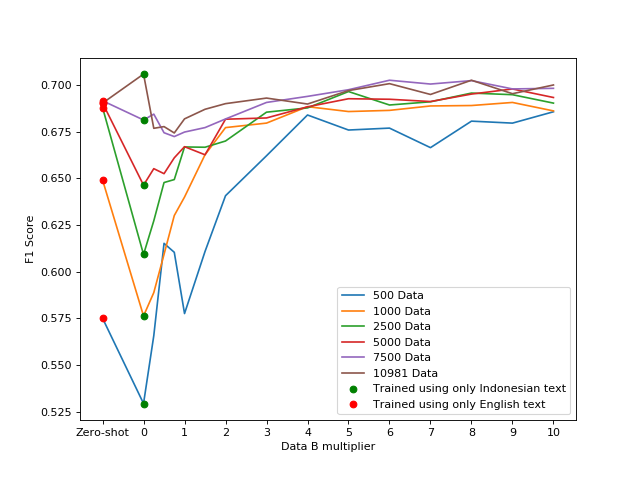
\includegraphics[width=\linewidth]{resources/plot-head-prosa-mbert.png}
            \caption{Plot dataset B model mBERT}
            \label{fig:plot_head_prosa_mbert}
            \endminipage\hfill
            \centering
            \minipage{0.33\paperwidth}
            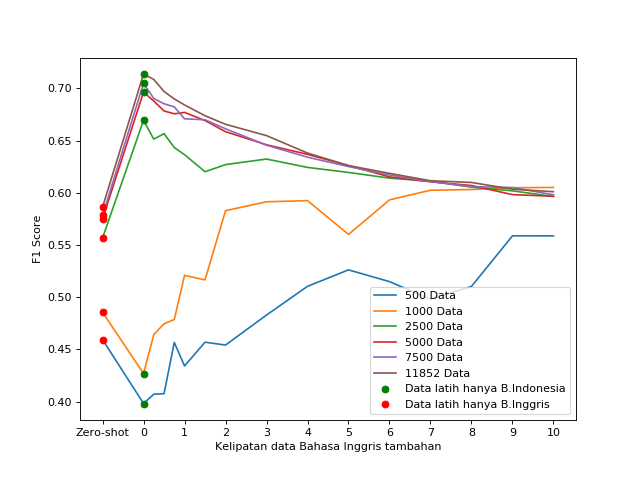
\includegraphics[width=\linewidth]{resources/plot-head-toxic-mbert.png}
            \caption{Plot ujaran kebencian model mBERT}
            \label{fig:plot_head_toxic_mbert}
            \endminipage
        \end{figure}

        \begin{enumerate}
            \item \textbf{Analisis sentimen dengan data dataset A} \\
            Dari Gambar \ref{fig:plot_head_trip_mbert}, ada beberapa poin yang dapat diobservasi:
            \begin{enumerate}
                \item Performa model secara general dibawah performa hasil model XLM-R.
                \item Performa zero-shot sangat buruk, semuanya dibawah 0.5.
                \item Pada jumlah data 500 \& 1000, model memiliki performa sangat buruk dan penambahan data bahasa Inggris tidak terlalu berarti.
                \item Pada jumlah data di atas 2500, penambahan data bahasa Inggris awalnya meningkatkan performa, tetapi berhenti seiring semakin besarnya jumlah data bahasa Inggris yang digunakan.
            \end{enumerate}

            % \begin{figure}[htb]
            %     \centering
            %     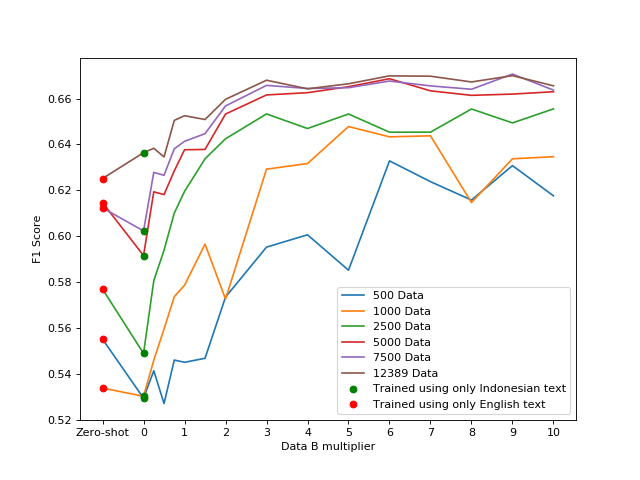
\includegraphics[width=\linewidth]{resources/plot-head-trip-mbert.png}
            %     \caption{Plot dataset A model mBERT}
            %     \label{fig:plot_head_trip_mbert}
            % \end{figure}
            

            \item \textbf{Analisis sentimen dengan dataset B} \\
            Dari Gambar \ref{fig:plot_head_prosa_mbert}, ada beberapa poin yang dapat diobservasi:
            \begin{enumerate}
                \item Performa model secara general dibawah performa hasil model XLM-R.
                \item Penambahan data bahasa Inggris awalnya meningkatkan performa, tetapi berhenti seiring semakin besarnya jumlah data yang digunakan.
            \end{enumerate}

            % \begin{figure}[htb]
            %     \centering
            %     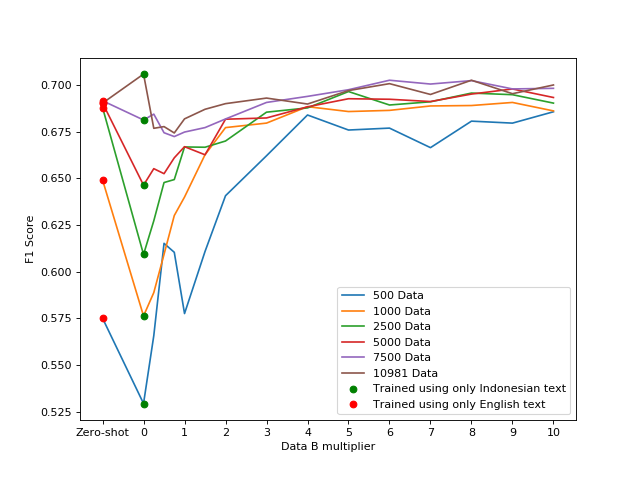
\includegraphics[width=\linewidth]{resources/plot-head-prosa-mbert.png}
            %     \caption{Plot dataset B model mBERT}
            %     \label{fig:plot_head_prosa_mbert}
            % \end{figure}
        
            \item \textbf{Klasifikasi ujaran kebencian \& kasar} \\
            Dari Gambar \ref{fig:plot_head_toxic_mbert}, ada beberapa poin yang dapat diobservasi:
            \begin{enumerate}
                \item Performa model secara general dibawah performa hasil model XLM-R.
                \item Penambahan data bahasa Inggris pada eksperimen dengan jumlah data 500 \& 1000  meningkatkan performa.
                \item Pada jumlah data di atas 2500, penambahan data bahasa Inggris langsung memperburuk performa model.
            \end{enumerate}

            % \begin{figure}[hbt]
            %     \centering
            %     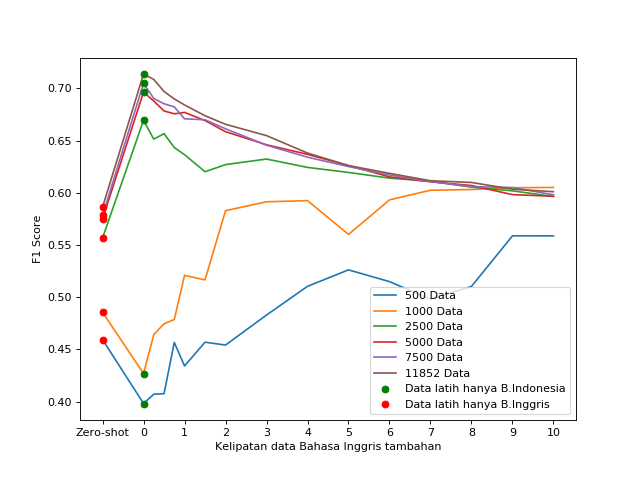
\includegraphics[width=\linewidth]{resources/plot-head-toxic-mbert.png}
            %     \caption{Plot ujaran kebencian model mBERT}
            %     \label{fig:plot_head_toxic_mbert}
            % \end{figure}

        \end{enumerate}

        Melalui rangkaian eksperimen dengan model mBERT pada gambar \ref{fig:plot_head_prosa_mbert}, \ref{fig:plot_head_trip_mbert}, dan \ref{fig:plot_head_toxic_mbert}, dapat dilihat bahwa secara umum performa model lebih buruk dibanding model XLM-R. Hal ini sudah diperkirakan. XLM-R dilatih dengan teknik yang lebih dioptimisasi untuk generalisasi antar bahasa dan data yang jauh lebih banyak. 
        
        Dengan merata-ratakan perbedaan antara nilai baseline monolingual dengan hasil tertinggi skenario \textit{multilingual learning}, tetap dapat dilihat dengan jelas efek penambahan data bahasa Inggris lebih tinggi di eksperimen dengan data bahasa Indonesia lebih sedikit. Hal ini kembali menunjukkan bahwasanya teknik ini lebih efektif jika jumlah data sedikit. Plot rata-rata dapat dilihat pada gambar \ref{fig:plot_gain_mbert}

        \begin{figure}[ht]
            \centering
            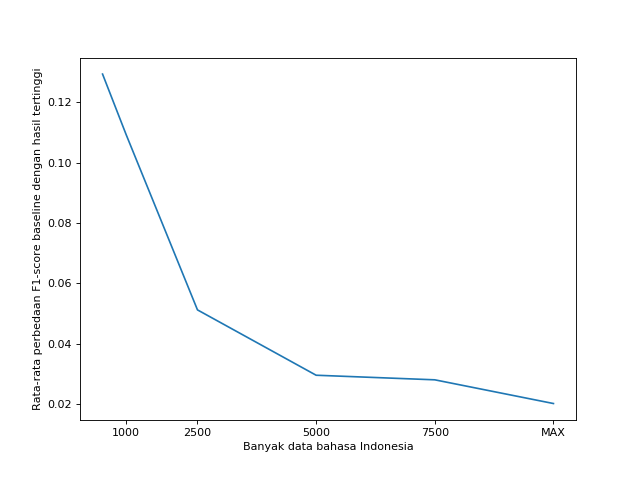
\includegraphics[width=0.9\textwidth]{resources/plot-gain-mbert.png}
            \caption{Plot rata-rata kenaikkan performa model mBERT}
            \label{fig:plot_gain}
        \end{figure}
        
        Selanjutnya, untuk melihat pemanfaatan \textit{multilingual language model} sepenuhnya dengan \textit{fine-tuning} penuh hanya model XLM-R yang akan dijalankan.

    \vspace{15mm}
    \subsection{Hasil fine-tuning penuh}
        Berikut hasil eksperimen \textit{fine-tuning} penuh model XLM-R pada analisis sentimen dan klasifikasi ujaran kebencian :
        \begin{enumerate}
            \item \textbf{Analisis sentimen dengan data dataset A} \\
            Dari Gambar \ref{fig:plot_full_trip_xlmr}, ada beberapa poin yang dapat diobservasi:
            \begin{enumerate}
                \item Performa model sangat bagus,. Pada eksperimen terbaik model mencapai F1-Score 0,893. Hal ini merupakan peningkatan dari penelitian sebelumnya yang mendapatkan F1-score 0,8341.
                \item Mengejutkan, performa terbaik dicapai oleh eksperimen zero-shot. Sedangkan performa model yang dilatih menggunakan bahasa Indonesia sangat rendah. Setelah melakukan inspeksi lebih lanjut ternyata dataset A memiliki 2573 teks duplikat. \\
                Dari total 12389 data teks, hanya 9816 teks yang unik. Hal ini menyebabkan \textit{language model} overfit kepada data ini dan tidak mempelajari permasalahan secara sepenuhnya. Pada subbab selanjutnya, eksperimen \textit{fine-tuning} penuh analisis sentimen data A dijalankan kembali pada dataset yang dihilangkan teks duplikatnya.
            \end{enumerate} 
             
            \begin{figure}[htb]
                \centering
                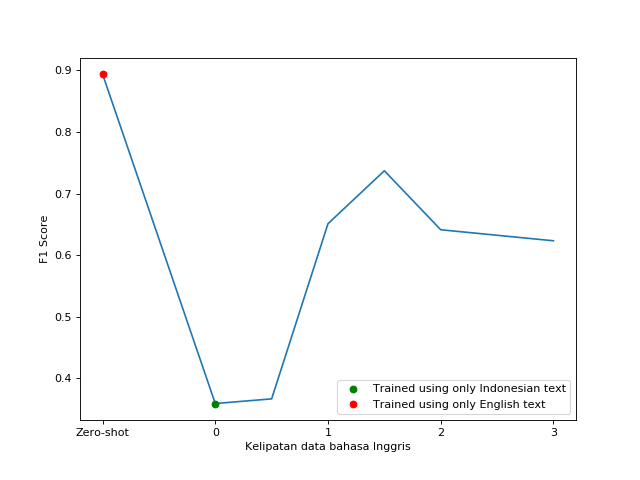
\includegraphics[width=0.9\textwidth]{resources/plot-full-trip-advisor-xlmr.png}
                \caption{Plot dataset A model XLM-R}
                \label{fig:plot_full_trip_xlmr}
            \end{figure}
            

            \item \textbf{Analisis sentimen dengan dataset B} \\
            Dari Gambar \ref{fig:plot_full_prosa_xlmr}, ada beberapa poin yang dapat diobservasi:
            \begin{enumerate}
                \item Performa model sangat bagus. Model berhasil memprediksi seluruh data tes dengan sempurna di skenario \textit{multilingual learning} dengan kelipatan bahasa Inggris 1.5. Hal ini merupakan peningkatan dari penelitian sebelumnya yang mendapatkan F1-score 0,9369.
                \item Performa model \textit{zero-shot}, berbeda dengan analisis sentimen pada dataset A, sangat buruk. Model mendapatkan F1-Score  0.335.
            \end{enumerate} 

            \begin{figure}[htb]
                \centering
                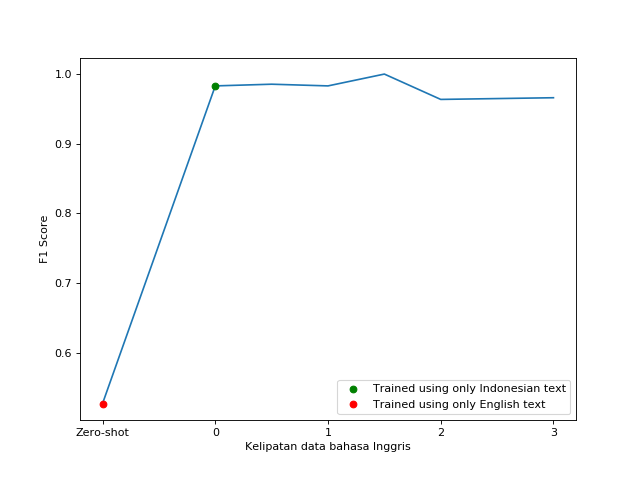
\includegraphics[width=0.9\textwidth]{resources/plot-full-prosa-xlmr.png}
                \caption{Plot dataset B model XLM-R}
                \label{fig:plot_full_prosa_xlmr}
            \end{figure}

         
            \item \textbf{Klasifikasi ujaran kebencian \& kasar} \\
            Dari Gambar \ref{fig:plot_full_toxic_xlmr}, ada beberapa poin yang dapat diobservasi:
            \begin{enumerate}
                \item Performa model sangat bagus. Model mendapatkan F1-score 0.898 dan akurasi 89.9\% pada eksperimen \textit{multilingual learning} dengan kelipatan data bahasa Inggris 3.
                \item Hingga akhir eksperimen dengan kelipatan data bahasa Inggris 3, model masih memperlihatkan peningkatan performa. Performa model dengan penambahan data bahasa Inggris masih dimungkinkan.
                \item  Penelitian sebelumnya yang menggunakan 3 label dan bukan yang disimplifikasi menjadi 2 seperti di penelitian ini. Pada subbab selanjutnya, eksperimen dijalankan dengan label mengikuti penelitian sebelumnya dan tanpa penambahan bahasa Inggris agar dapat dibandingkan.
            \end{enumerate} 

            \begin{figure}[htb]
                \centering
                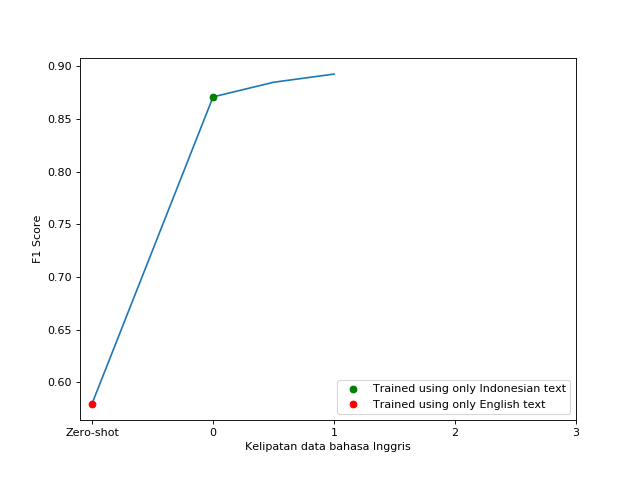
\includegraphics[width=0.9\textwidth]{resources/plot-full-toxic-xlmr.png}
                \caption{Plot Ujaran kebencian model XLM-R}
                \label{fig:plot_full_toxic_xlmr}
            \end{figure}

        \end{enumerate}

        Melalui eksperimen \textit{fine-tuning} penuh dengan model XLM-R, dapat dilihat performa model XLM-R sangat bagus pada analisis sentimen dataset B dan klasifikasi ujaran kebencian. Meski begitu, pada analisis sentimen dataset A, model yang dilatih dengan bahasa Indonesia dan campuran memiliki performa yang jauh lebih jelek dibanding model yang dilatih dengan bahasa Inggris saja. Selain itu, hasil \textit{fine-tuning} penuh klasifikasi ujaran kebencian tidak dapat dibandingkan dengan penelitian sebelumnya secara langsung. Dua hal ini dibahas pada bab selanjutnya

\section{Analisis Hasil Tambahan}
    Subbab ini membahas lebih detail hasil yang didapatkan pada bab sebelumnya.
    
    \subsection{Hasil fine-tuning penuh klasifikasi ujaran kebencian yang dapat dibandingkan}
        Untuk dapat membandingkan secara langsung penggunaan \textit{multilingual language model}, pelatihan dengan konfigurasi yang sama dengan skenario 2 penelitian \parencite{Ibrohim_Budi_2019} dilakukan. Dapat dilihat pada Tabel \ref{tab:toxic_xlm_r_comparable}, model mendapatkan rata-rata akurasi 89.52\%. Hal ini merupakan peningkatan dari penelitian sebelumnya yang mendapatkan \textit{average accuracy} tertinggi 77.36\%.

        \begin{table}[htb]
            \centering
            \caption{Hasil \textit{fine-tuning} penuh klasifikasi ujaran kebencian \textit{comparable}}
            \begin{tabular}{|r|l|l|l|}
            \hline
            \multicolumn{1}{|l|}{} & \textbf{Hate Speech} & \textbf{Abusive} & \textbf{Average}      \\ \hline
            \textbf{Accuracy}      & 85.573273\%          & 93.470008\%      & \textbf{89.5216405\%} \\ \hline
            \textbf{F1}            & 0.85331737           & 0.93094791       & \textbf{0.89213264}   \\ \hline
            \end{tabular}
            
            \label{tab:toxic_xlm_r_comparable}
        \end{table}

        

    \subsection{Hasil fine-tuning penuh analisis sentimen dataset A tanpa duplikat}
        Setelah ditelusuri, ternyata dataset A memiliki 2573 teks duplikat. Sehingga, dari total 12389 data teks, hanya 9816 teks yang unik. Hal ini menyebabkan \textit{language model} overfit kepada data ini dan tidak mempelajari permasalahan secara sepenuhnya. Eksperimen \textit{fine-tuning} penuh analisis sentimen data A dijalankan kembali pada dataset yang dihilangkan teks duplikatnya. Hasilnya dapat dilihat pada Gambar \ref{fig:plot_fuLL_trip_duplicate}

        \begin{figure}[htb]
            \centering
            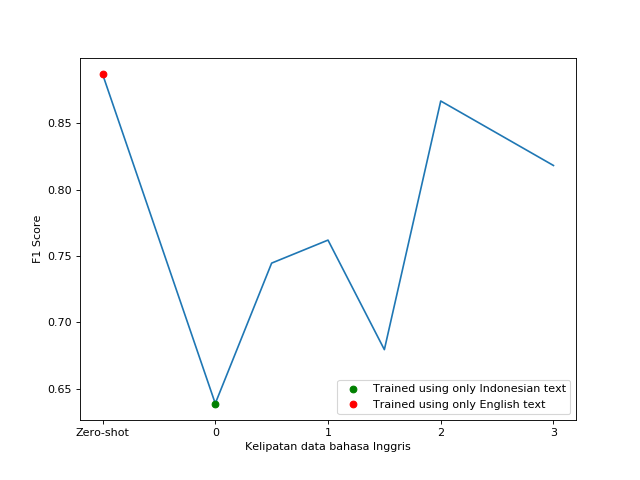
\includegraphics[width=0.9\linewidth]{resources/plot-full-trip-advisor-xlmr-duplicate.png}
            \caption{Plot dataset A model XLM-R duplikat dihilangkan}\label{fig:plot_fuLL_trip_duplicate}
        \end{figure}

        Dapat dilihat dari Gambar \ref{fig:plot_fuLL_trip_duplicate}, performa model pada eksperimen yang menggunakan bahasa Indonesia membaik. Tetapi hasil terbaik tetap pada eksperimen \textit{zero-shot} dengan besar F1-score 0.886. Penelitian sebelumnya oleh \parencite{FarhanKhodra2017} tetap menggunakan data seluruhnya dan tidak menghilangkan duplikat. Oleh karena itu, pada kesimpulan akhir hasil eksperimen tanpa menghilangkan data duplikat yang akan dibandingkan.
    
        

    \subsection{Analisis Kasus Peningkatan Performa}
        Pada kasus fine-tuning penuh analisis sentimen dataset B, terdapat 8 data yang sebelumnya salah diprediksi pada eksperimen monolingual dan berhasil diprediksi pada eksperimen multilingual. Menariknya dari delapan data tersebut, semuanya bahasa Indonesia. Hal ini memperlihatkan penambahan data bahasa Inggris dapat membantu model mendapatkan informasi baru dalam bahasa Indonesia. Contoh dapat dilihat pada Tabel \ref{tab:case_improvement}.

        \begin{table}[htb]
            \centering
            \caption{Analisis kasus peningkatan performa}
            \begin{tabular}{|l|l|r|r|r|}
            \hline
            \multicolumn{1}{|c|}{\textbf{No}} & \multicolumn{1}{c|}{\textbf{Teks}}                                                                        & \multicolumn{1}{c|}{\textbf{Label}} & \multicolumn{1}{c|}{\textbf{\begin{tabular}[c]{@{}c@{}}Prediksi \\ Monolingual\end{tabular}}} & \multicolumn{1}{c|}{\textbf{\begin{tabular}[c]{@{}c@{}}Prediksi \\ Multilingual\end{tabular}}} \\ \hline
            1                                 & produk lokal memang cetek                                                                                 & 0                                   & 0.85668                                                                                       & 0.05138                                                                                        \\ \hline
            2                                 & \begin{tabular}[c]{@{}l@{}}gila sih rasa iga bakar di iga \\ bakar si jangkung terbaik parah\end{tabular} & 1                                   & 0.01425                                                                                       & 0.99666                                                                                        \\ \hline
            \end{tabular}
            \label{tab:case_improvement}
        \end{table}

